\documentclass[12pt,a4paper]{ctexart}
\usepackage[margin=2.2cm]{geometry}
\usepackage{booktabs}
\usepackage{array}
\usepackage{longtable}
\usepackage{float}
\usepackage{caption}
\usepackage{hyperref}
\usepackage{siunitx}
\usepackage{amsmath,amssymb}

\title{补充材料\\PTMC 中央区淋巴结转移临床论文重组稿}
\author{PTMC-LNM Study Group}
\date{\today}

\begin{document}
\maketitle

\section{补充说明}
本补充材料保留主文未展开的详细结果，主要包括三部分：原始临床回归的完整三任务汇总、历史版本消融逐折明细（含 Base-A），以及多源融合多版本比较（含 EffNet-B0 与 ViT-B/16 的方法学对照）。早期排查型实验、日志可信度修复和开发过程记录未纳入最终稿件，也不在本补充材料中重复展开。

\section{原始临床回归的完整三任务结果}
\begin{table}[H]
\centering
\caption{原始临床回归基线的三任务结果汇总（患者级 5-fold）}
\label{tab:supp_raw_clinical_all}
\small
\begin{tabular}{lccccc}
\toprule
任务 & AUC Mean$\pm$Std & ACC & F1 & Sen & Spe \\
\midrule
LNM & $0.7023\pm0.0448$ & 0.6356 & 0.6705 & 0.6721 & 0.5880 \\
CentralLNM & $0.6859\pm0.0658$ & 0.6332 & 0.6661 & 0.6712 & 0.5881 \\
LateralLNM & $0.8409\pm0.0902$ & 0.9094 & 0.3055 & 0.2818 & 0.9720 \\
\bottomrule
\end{tabular}
\end{table}

\section{历史版本六组消融的逐折结果（含 Base-A）}
\begin{table}[H]
\centering
\small
\caption{Per-fold metrics: Baseline A (Clinical-only)}
\label{tab:baseline_a_clinical_only_per_fold}
\begin{tabular}{rrrrrr}
\toprule
fold & AUC & ACC & F1 & Sen & Spe \\
\midrule
0 & 0.640 & 0.563 & 0.513 & 0.426 & 0.725 \\
1 & 0.711 & 0.690 & 0.703 & 0.681 & 0.700 \\
2 & 0.632 & 0.547 & 0.589 & 0.596 & 0.487 \\
3 & 0.652 & 0.581 & 0.581 & 0.532 & 0.641 \\
4 & 0.702 & 0.671 & 0.745 & 0.891 & 0.410 \\
\bottomrule
\end{tabular}
\end{table}

\begin{table}[H]
\centering
\small
\caption{Per-fold metrics: Baseline B (Slice-Mean + Concat)}
\label{tab:baseline_b_slice_mean_concat_per_fold}
\begin{tabular}{rrrrrr}
\toprule
fold & AUC & ACC & F1 & Sen & Spe \\
\midrule
0 & 0.662 & 0.632 & 0.704 & 0.809 & 0.425 \\
1 & 0.657 & 0.540 & 0.630 & 0.723 & 0.325 \\
2 & 0.653 & 0.640 & 0.687 & 0.723 & 0.538 \\
3 & 0.661 & 0.570 & 0.602 & 0.596 & 0.538 \\
4 & 0.721 & 0.600 & 0.691 & 0.826 & 0.333 \\
\bottomrule
\end{tabular}
\end{table}

\begin{table}[H]
\centering
\small
\caption{Per-fold metrics: Ablation 1 (Mean-MIL + Gated)}
\label{tab:ablation1_mean_mil_gated_per_fold}
\begin{tabular}{rrrrrr}
\toprule
fold & AUC & ACC & F1 & Sen & Spe \\
\midrule
0 & 0.675 & 0.621 & 0.645 & 0.638 & 0.600 \\
1 & 0.708 & 0.644 & 0.680 & 0.702 & 0.575 \\
2 & 0.624 & 0.593 & 0.568 & 0.489 & 0.718 \\
3 & 0.669 & 0.616 & 0.560 & 0.447 & 0.821 \\
4 & 0.713 & 0.659 & 0.707 & 0.761 & 0.538 \\
\bottomrule
\end{tabular}
\end{table}

\begin{table}[H]
\centering
\small
\caption{Per-fold metrics: Ablation 2 (Attention-MIL + Concat)}
\label{tab:ablation2_attention_mil_concat_per_fold}
\begin{tabular}{rrrrrr}
\toprule
fold & AUC & ACC & F1 & Sen & Spe \\
\midrule
0 & 0.637 & 0.609 & 0.679 & 0.766 & 0.425 \\
1 & 0.705 & 0.655 & 0.659 & 0.617 & 0.700 \\
2 & 0.654 & 0.593 & 0.653 & 0.702 & 0.462 \\
3 & 0.641 & 0.605 & 0.605 & 0.553 & 0.667 \\
4 & 0.700 & 0.612 & 0.686 & 0.783 & 0.410 \\
\bottomrule
\end{tabular}
\end{table}

\begin{table}[H]
\centering
\small
\caption{Per-fold metrics: Ablation 3 (No Prior Constraint)}
\label{tab:ablation3_no_penalty_per_fold}
\begin{tabular}{rrrrrr}
\toprule
fold & AUC & ACC & F1 & Sen & Spe \\
\midrule
0 & 0.693 & 0.598 & 0.588 & 0.532 & 0.675 \\
1 & 0.690 & 0.552 & 0.678 & 0.872 & 0.175 \\
2 & 0.625 & 0.581 & 0.600 & 0.574 & 0.590 \\
3 & 0.665 & 0.593 & 0.607 & 0.574 & 0.615 \\
4 & 0.686 & 0.612 & 0.718 & 0.913 & 0.256 \\
\bottomrule
\end{tabular}
\end{table}

\begin{table}[H]
\centering
\small
\caption{Per-fold metrics: Ours (Attention-MIL + Gated + Prior)}
\label{tab:ours_full_per_fold}
\begin{tabular}{rrrrrr}
\toprule
fold & AUC & ACC & F1 & Sen & Spe \\
\midrule
0 & 0.680 & 0.598 & 0.632 & 0.638 & 0.550 \\
1 & 0.691 & 0.563 & 0.667 & 0.809 & 0.275 \\
2 & 0.699 & 0.663 & 0.695 & 0.702 & 0.615 \\
3 & 0.715 & 0.663 & 0.713 & 0.766 & 0.538 \\
4 & 0.696 & 0.635 & 0.667 & 0.674 & 0.590 \\
\bottomrule
\end{tabular}
\end{table}


\section{多源融合多版本比较（方法学补充）}
\begin{table}[H]
\centering
\caption{EffNet-B0：V1 与三种 V2 融合版本对比（患者级 5-fold，历史方法学补充）}
\small
\begin{tabular}{lccccccc}
\toprule
版本 & AUC$_{cen}$ & AUC$_{lnm}$ & ACC & F1 & Sen & Spe & Compliance \\
\midrule
V1 & $0.6732\pm0.0236$ & $0.6992\pm0.0110$ & 0.6173 & 0.6592 & 0.7014 & 0.5178 & $0.9700\pm0.0382$ \\
V2-legacy & $0.6708\pm0.0544$ & $0.7032\pm0.0388$ & 0.6426 & 0.6826 & 0.7096 & 0.5632 & $0.9603\pm0.0311$ \\
V2-align\_proj & $0.6911\pm0.0323$ & $0.7037\pm0.0257$ & 0.6034 & 0.6228 & 0.6290 & \textbf{0.5744} & $0.9608\pm0.0408$ \\
V2-FiLM & $\mathbf{0.6951\pm0.0354}$ & $0.6978\pm0.0323$ & 0.6333 & \textbf{0.6930} & \textbf{0.7607} & 0.4826 & $\mathbf{0.9747\pm0.0303}$ \\
\bottomrule
\end{tabular}
\end{table}

\begin{table}[H]
\centering
\caption{Swin-T：V1 与三种 V2 融合版本对比（患者级 5-fold）}
\small
\begin{tabular}{lccccccc}
\toprule
版本 & AUC$_{cen}$ & AUC$_{lnm}$ & ACC & F1 & Sen & Spe & Compliance \\
\midrule
V1 & $\mathbf{0.6939\pm0.0267}$ & $\mathbf{0.7011\pm0.0203}$ & \textbf{0.6473} & \textbf{0.6620} & 0.6635 & \textbf{0.6296} & $\mathbf{0.9977\pm0.0047}$ \\
V2-legacy & $0.6793\pm0.0313$ & $0.6914\pm0.0343$ & 0.6263 & 0.6601 & \textbf{0.6709} & 0.5736 & $0.9348\pm0.0853$ \\
V2-align\_proj & $0.6646\pm0.0434$ & $\mathbf{0.7015\pm0.0453}$ & 0.5942 & 0.6264 & 0.6325 & 0.5499 & $0.9723\pm0.0237$ \\
V2-FiLM & $0.6631\pm0.0399$ & $0.6679\pm0.0326$ & 0.6009 & 0.6278 & 0.6424 & 0.5514 & $0.9724\pm0.0440$ \\
\bottomrule
\end{tabular}
\end{table}

\begin{table}[H]
\centering
\caption{ViT-B/16：V1 与三种 V2 融合版本对比（患者级 5-fold）}
\small
\begin{tabular}{lccccccc}
\toprule
版本 & AUC$_{cen}$ & AUC$_{lnm}$ & ACC & F1 & Sen & Spe & Compliance \\
\midrule
V1 & $\mathbf{0.7104\pm0.0253}$ & $\mathbf{0.7222\pm0.0295}$ & 0.6289 & 0.6686 & 0.6969 & 0.5490 & $0.9512\pm0.0626$ \\
V2-legacy & $0.6404\pm0.0496$ & $0.6592\pm0.0522$ & 0.5779 & 0.6478 & \textbf{0.7220} & 0.4077 & $0.9398\pm0.0621$ \\
V2-align\_proj & $0.6971\pm0.0356$ & $0.7155\pm0.0217$ & 0.6403 & 0.6505 & 0.6327 & \textbf{0.6495} & $0.9561\pm0.0601$ \\
V2-FiLM & $0.6868\pm0.0451$ & $0.6991\pm0.0451$ & \textbf{0.6428} & \textbf{0.6706} & 0.6663 & 0.6149 & $\mathbf{0.9837\pm0.0158}$ \\
\bottomrule
\end{tabular}
\end{table}

\section{代表性病例可视化补充}
为补充主文中的可解释性证据，本节给出中风险与低风险代表病例在“多切面”与“多模态”两个维度的 Grad-CAM 可视化。

\begin{figure}[H]
  \centering
  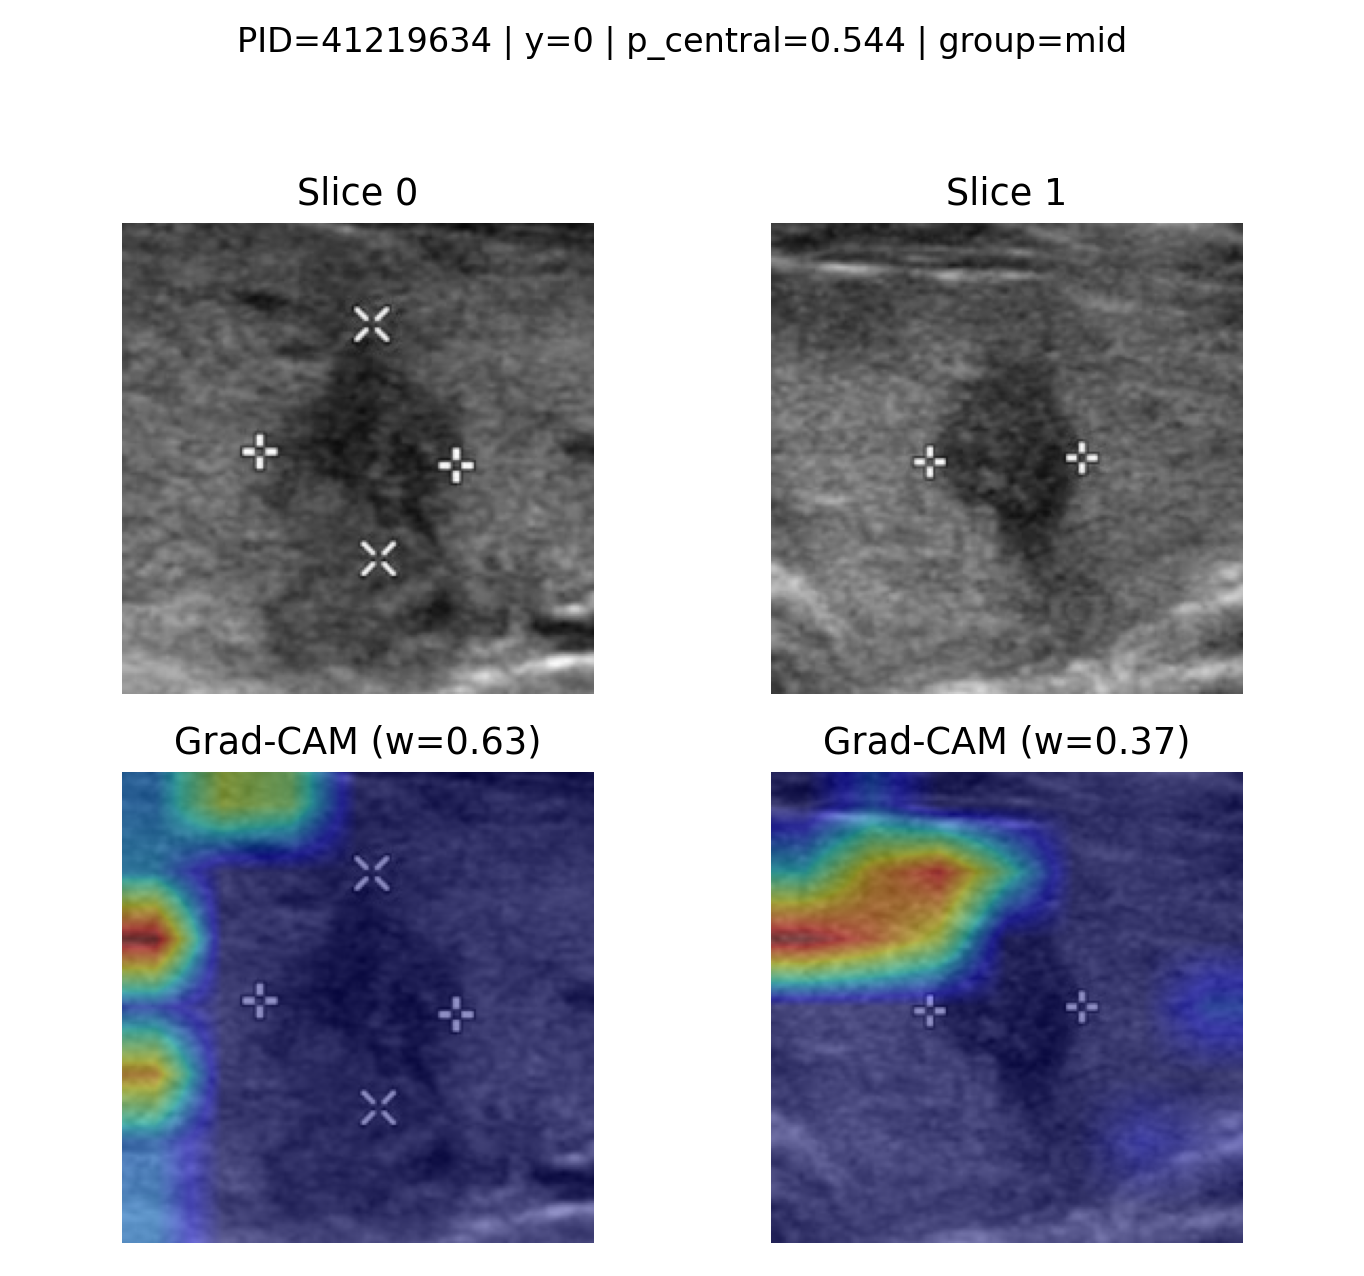
\includegraphics[width=0.90\textwidth]{figures/gradcam_slices_case_mid.png}
  \caption{中风险代表病例的多切面 Grad-CAM 可视化。可见激活区域在切面间存在明显异质性，提示模型对该类病例依赖少数关键切面进行判别。}
\end{figure}

\begin{figure}[H]
  \centering
  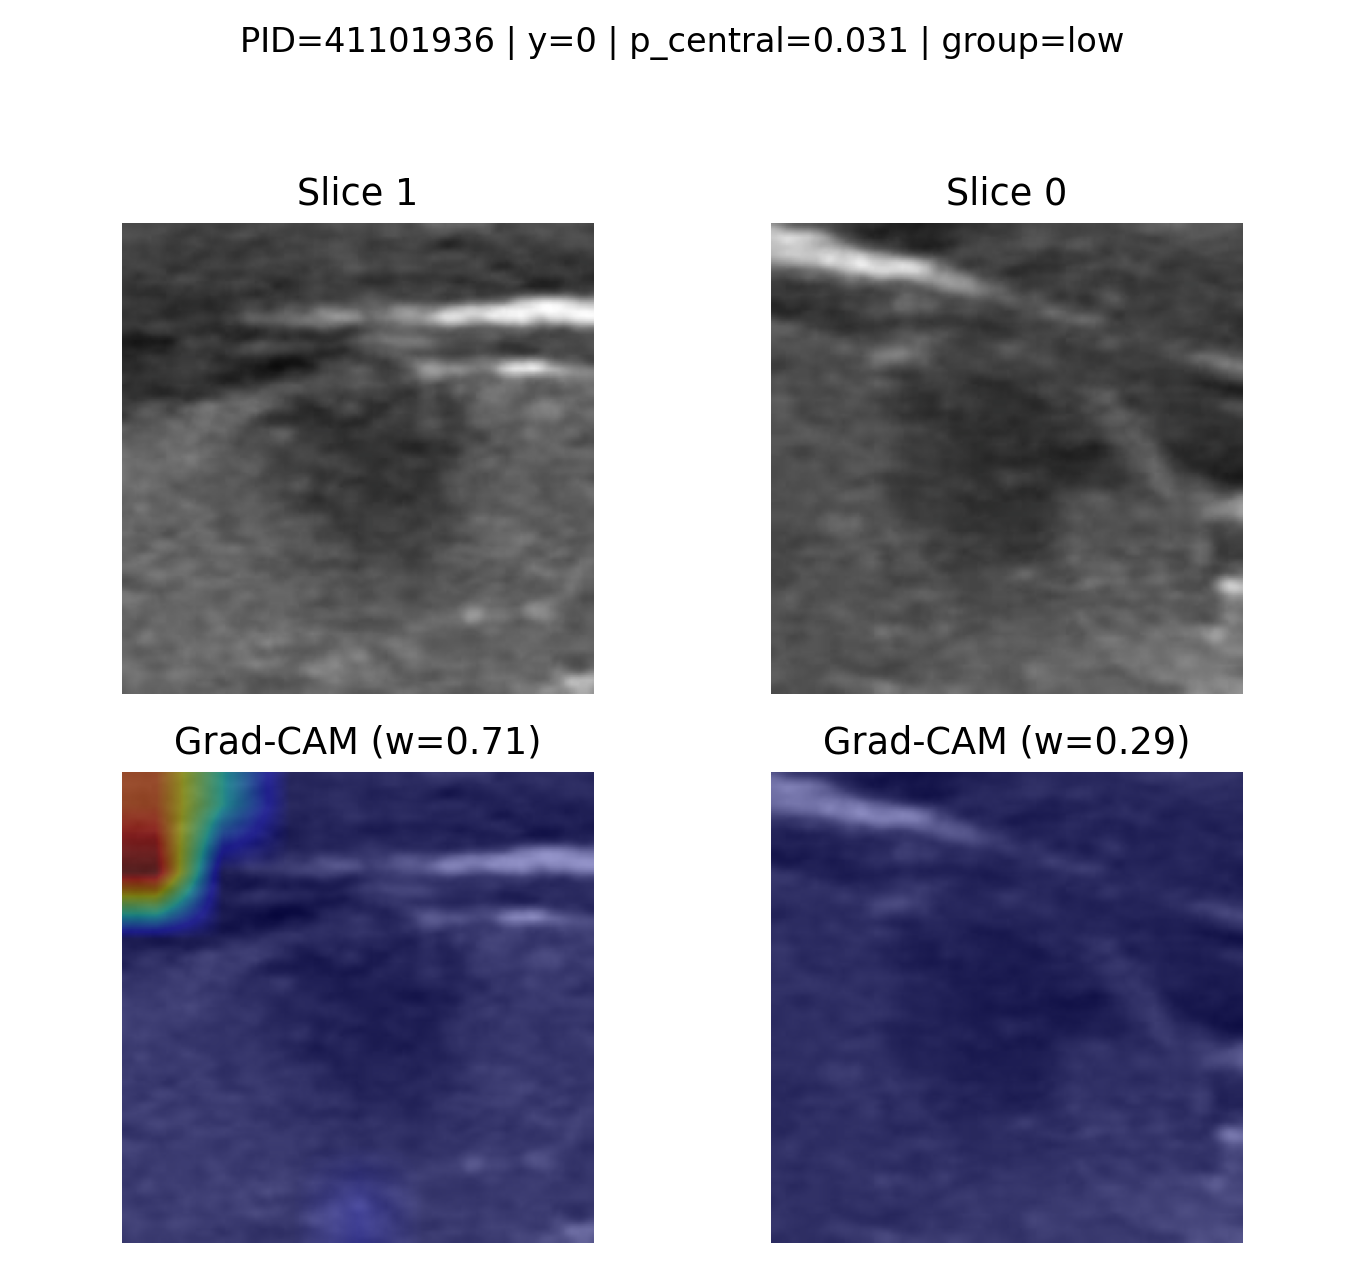
\includegraphics[width=0.90\textwidth]{figures/gradcam_slices_case_low.png}
  \caption{低风险代表病例的多切面 Grad-CAM 可视化。整体激活强度较弱且分布更分散，与低风险预测结果一致。}
\end{figure}

\begin{figure}[H]
  \centering
  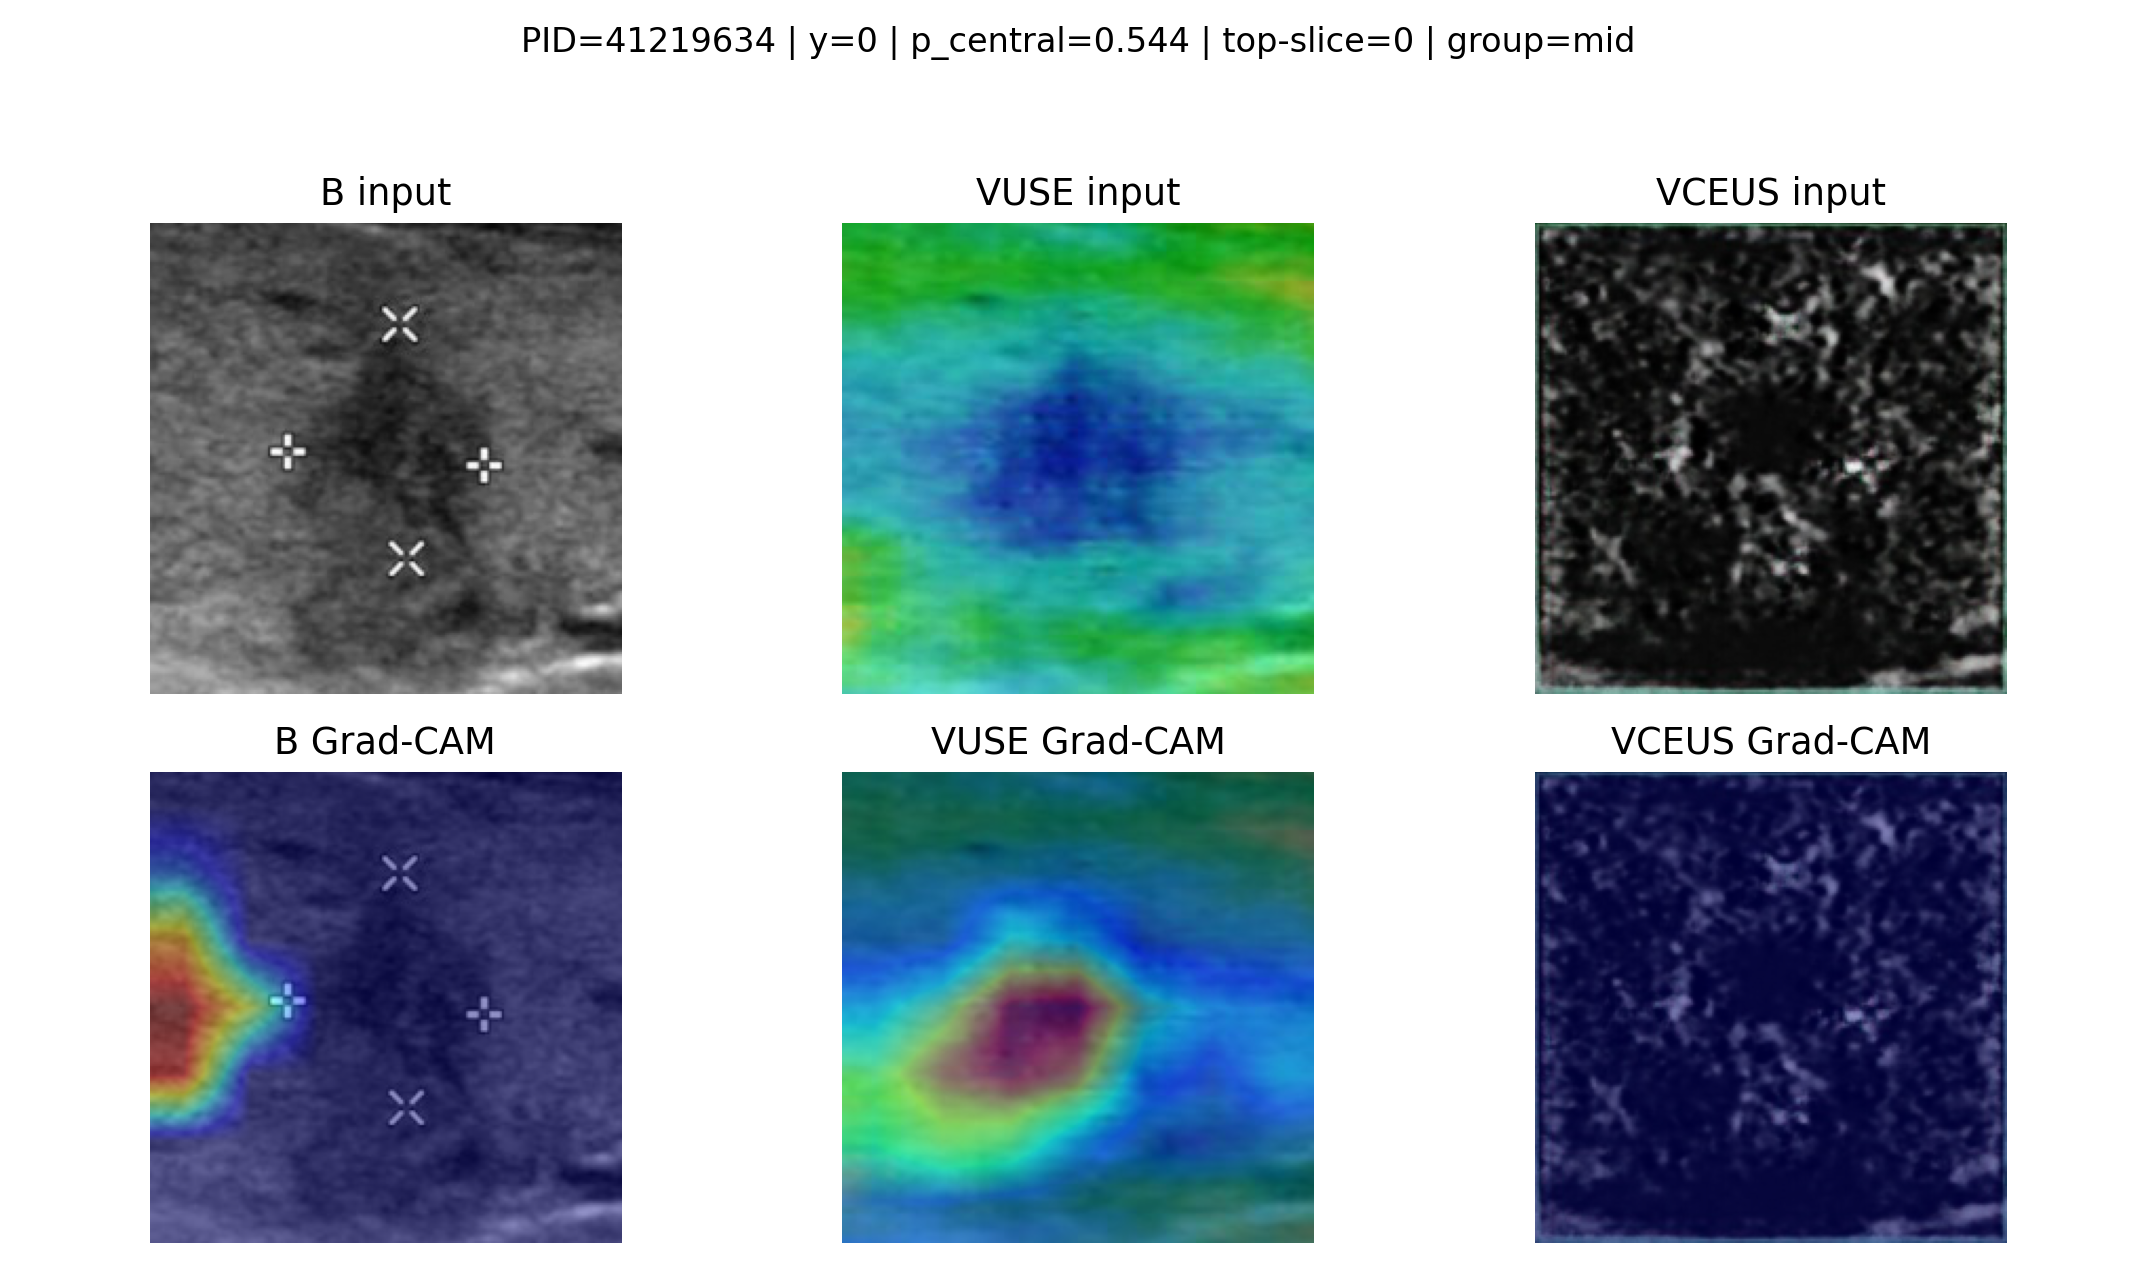
\includegraphics[width=0.90\textwidth]{figures/gradcam_modalities_case_mid.png}
  \caption{中风险代表病例的多模态 Grad-CAM 可视化。不同模态在相同解剖区域的响应程度存在差异，提示模态间互补可能主要体现在边界病例。}
\end{figure}

\begin{figure}[H]
  \centering
  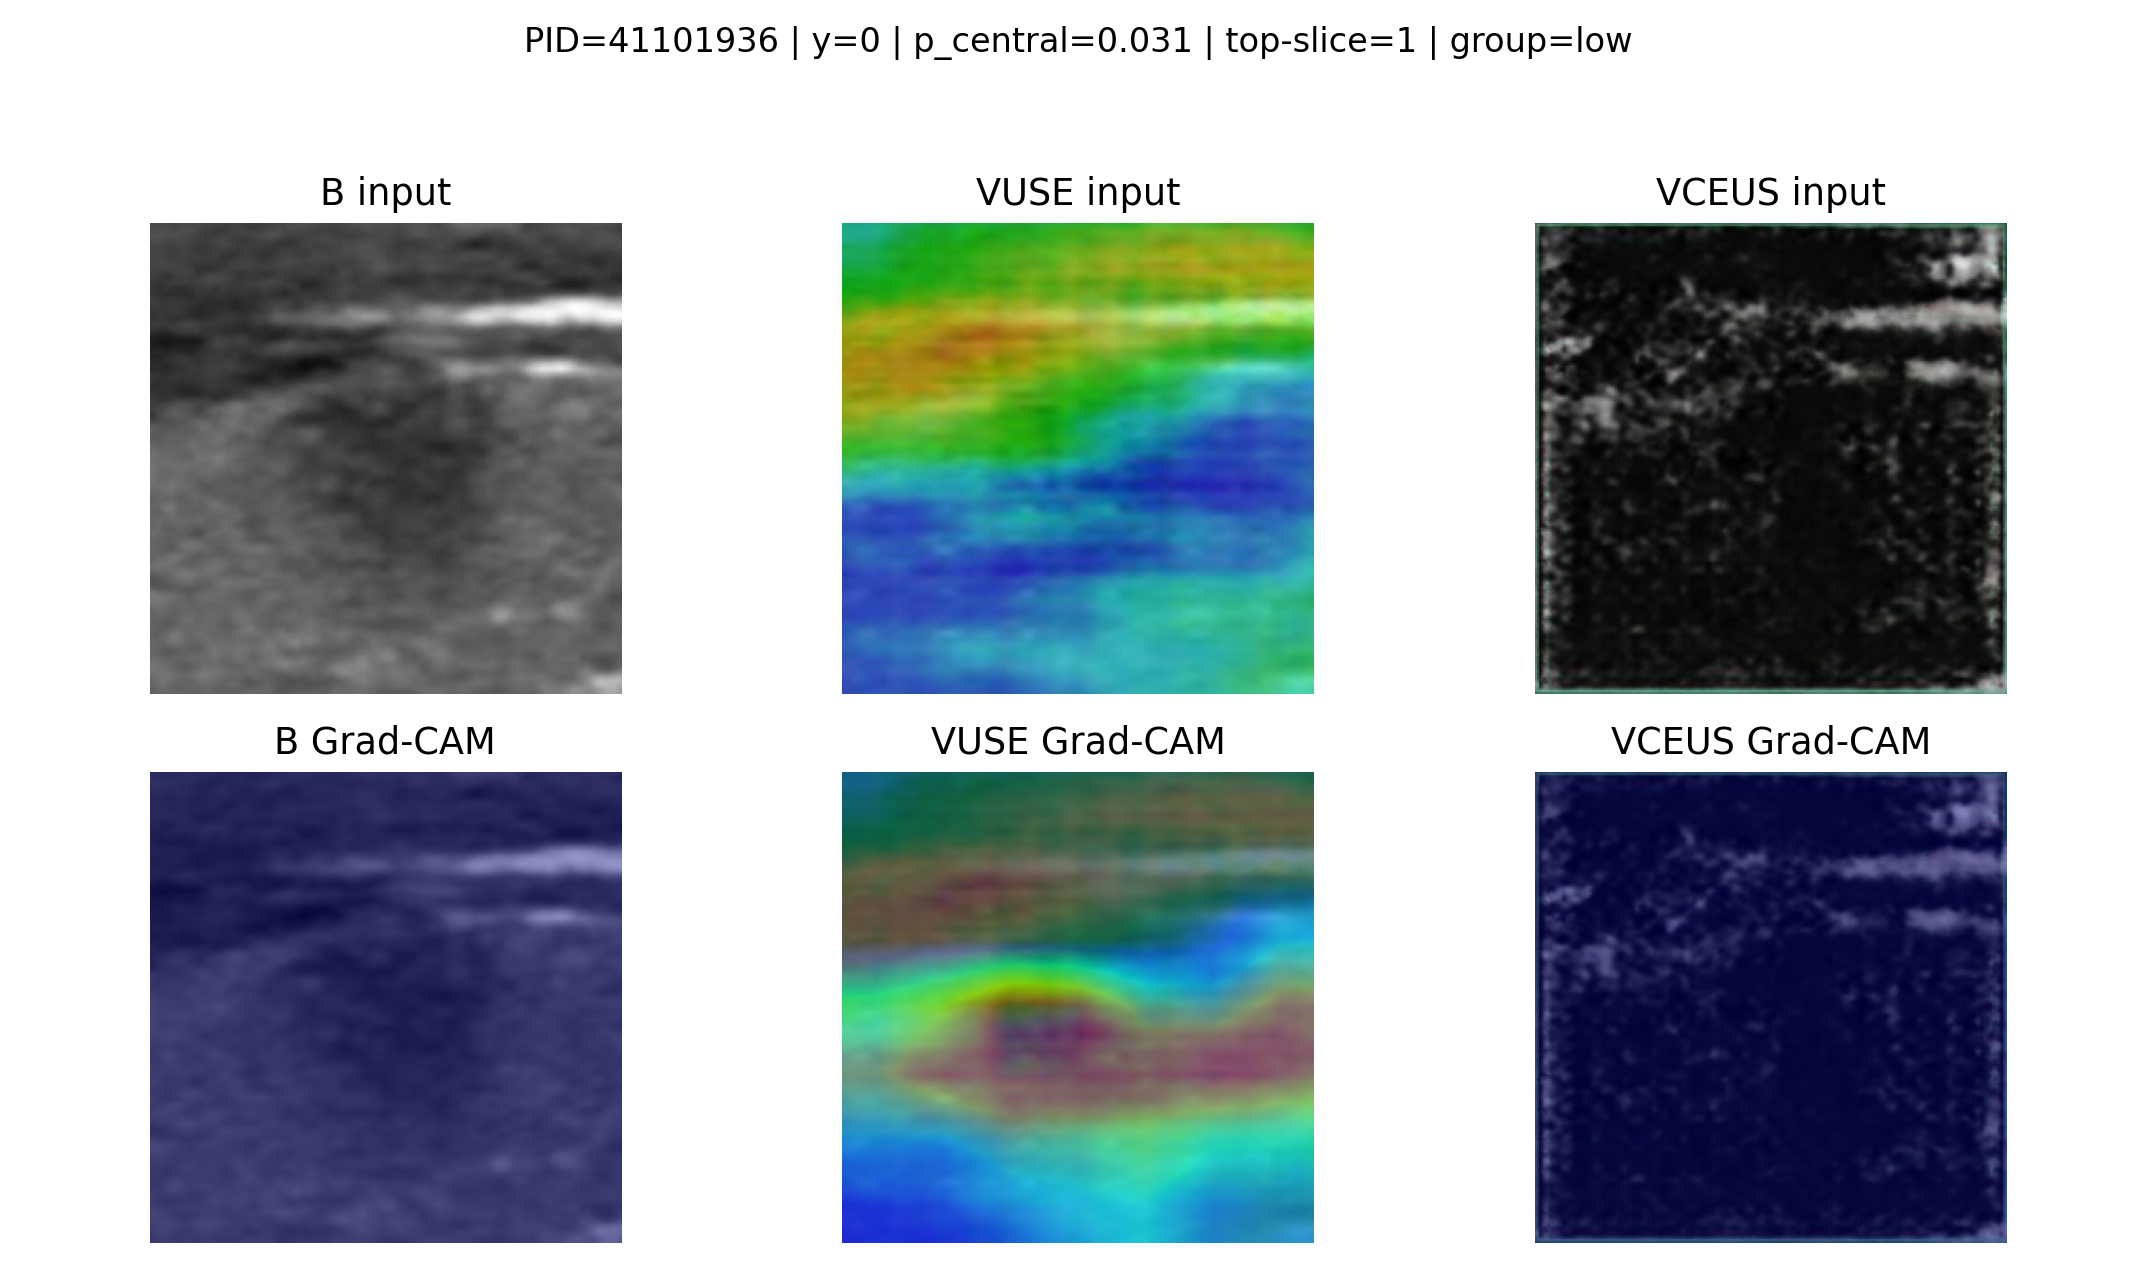
\includegraphics[width=0.90\textwidth]{figures/gradcam_modalities_case_low.png}
  \caption{低风险代表病例的多模态 Grad-CAM 可视化。各模态均未出现持续高强度聚焦区域，支持模型对低风险样本的保守判断。}
\end{figure}

\paragraph{补充解释}
上述可视化与主文定量结果方向一致：高风险病例通常呈现更集中的激活区域，中低风险病例则表现为更分散或更弱的响应；模态间差异在中风险病例中更明显，提示多模态融合对边界病例判别可能更具价值。

\section{补充结论}
补充结果进一步说明，多源融合的表现具有明显骨干依赖性：EffNet-B0 在 FiLM 下获益更明显，ViT-B/16 在对齐投影策略下恢复更好，而 Swin-T 在当前两种新融合器下均未优于 legacy 版本。该结论用于说明不同融合策略的适用边界，不改变主文采用 ViT-B/16 作为核心结果版本的结论。

\end{document}
